\section{Simple model} \slabel{model}

We base our model on the buoyancy-drag models of \cite{Oron2001}:
\begin{equation}
(\rho_1 + \rho_2) \mathcal{V} \ddot{h} = (\rho_2 - \rho_1) \mathcal{V} - C \dot{h}^2 \rho \mathcal{A}
\end{equation}
where $\rho_1$ and $\rho_2$ are the densities of the light and heavy fluid,
$\mathcal{V}$ is the characteristic volume of the bubble
$g$ is the acceleration,
$C$ is a drag-like coefficient, and
$\mathcal{A}$ is the characteristic cross sectional area of the bubble.
Making the Boussinesq approximation, $\rho_1 \approx \rho_2$ yields:
\begin{equation}
\ddot{h} = A g - \frac{C}{2} \dot{h}^2 \frac{\mathcal{A}}{\mathcal{V}}
\end{equation}
In the self-similar regime there is only one length-scale, so $\mathcal{A}/\mathcal{V} \sim 1 / \lambda$.
However, in the single-mode regime that is the focus of this study, the bubbles are elongated, producing two length scales: a span-wise scale $\lambda$ and a stream-wise scale $h$.
Therefore, for the smRTI $\mathcal{A}/\mathcal{V} \sim \frac{1}{h}$ and the model of Oron et. al yields un-bounded velocities:
\begin{equation}
\ddot{h} = A g - \frac{C}{2} \frac{\dot{h}^2}{h}
\end{equation}
Because the strength of the form drag relative to buoyancy decreases at high aspect ratio, we must consider other drag terms, such as skin drag, that grow at least linearly with $h$.

\subsection{Dynamics}

We begin by listing the external forces the bubble experiences.  The first is the buoyant force:
\begin{equation}
F_b = C_0 A g \lambda^2 h,
\end{equation}
where $C_0$ is an unknown coefficient.
The next is the form drag:
\begin{equation}
F_f = C_1 \lambda^2 \dot{h}^2,
\end{equation}
where $C_1$ is similar to a drag coefficient.
The next is the viscous, or skin, drag:
\begin{equation}
F_s = C_2 \nu h \dot{h},
\end{equation}
where $C_2$ is another unknown coefficient and 
$\nu$ is the kinematic vicosity.

To complete the dynamic equation, we must characterize the inertia of the bubble.
The bubble is roughly cylindrical with a height $h$, so we expect an inertial term of the form $\lambda^2 h$.
However, consider the limit of $h \rightarrow 0$.  
Here, streamlines must extend from bubble to spike, which has a characteristic separation $\lambda$ for an inertial term of the form $\lambda^3$.
Therefore, we expect the inertia to be a mix of a term that goes as $\lambda^2 h$ and one that goes as$\lambda^3$:
\begin{equation} \elabel{inertia}
I = C_4 \lambda^2 h + C_3 \lambda^3,
\end{equation}
where $C_4$ and $C_5$ are two more unknown coefficients.

The complete dynamic equation is:
\begin{equation}
\ddot{h} = \frac{C_0 A g \lambda^2 h - C_1 \lambda^2 \dot{h}^2 - C_2 \nu h \dot{h}}{C_3 \lambda^2 h + C_4 \lambda^3}
\end{equation}
Without loss of generality, we can let $C_0 = 1$ and simplify:
\begin{equation}
\ddot{h} = \frac{A g h - C_1 \dot{h}^2 - C_2 \nu (h/\lambda) \dot{h}}{ C_3 h + C_4 \lambda }
\end{equation}
We can non-dimensionalize by defining a dimensionless length and time:
\begin{equation}
z = \frac{h}{\lambda} \qquad \tau = \sqrt{\frac{A g}{\lambda}} t,
\end{equation}
which simplifes:
\begin{equation}
\ddot{z} = \frac{z - C_1 \dot{z}^2 - C_2 \text{Gr}^{-1/2} z \dot{z}}{C_3 z + C_4},
\end{equation}
where $\text{Gr} = A g \lambda^3 \nu^{-2}$ is the Grashof number.


\subsection{Mixing}

As the bubble height grows, the velocity approaches a terminal value specified by the balance between buoyancy and skin drag.
At terminal velocity, the flux of pure fluid into the bubble is bounded.
However, the interfacial mixing continues to grow with the interfacial area, which grows with $h$.
Therefore, for any finite diffusivity, the bubble will ultimately diffuse away.
For this reason, we must include the effects of interficial mixing, at least to the first order.

The quantity of mixed fluid, $M$ is computed directly from the time, bubble height, diffusivity, and initial interface thicnkess.
The quantity of mixed fluid is defined as the integral of the absolute value of the scalar:
\begin{equation}
M(t) = \int 1-\text{abs}\left[\phi(x,y,z,t)\right] dV,
\end{equation}
where we assume the mean scalar is zero, $\int \phi dV = 0$.

We approximate the volume integral by a 1D integral across the interface multiplied by the surface area:
\begin{equation}
M(t) \approx S \int 1- \text{abs}\left[\phi_1(r)\right] dr
\end{equation}
where $S$ is the surface area and
$\phi_1$ is a model 1D scalar profile:
\begin{equation}
\phi_1(r) = \frac{1}{2} \left( \erf\left[\frac{r}{\delta}\right] - \erf\left[\frac{r - d}{\delta}\right] \right),
\end{equation}
where $\delta$ is the interface width and
$d$ is the diameter of the bubble.

The surface area has contributions from the bubble tip and side walls:
\begin{equation}
S = \left(C_6 \lambda^2 + C_5 \lambda h\right)
\end{equation}
where $C_5$ and $C_6$ are unknown coefficients.
$C_5$ scales the perimeter of span-wise slices of the bubble while $C_6$ rescales bubble tip.

To the first order, the diameter is half the wavelength: $d \approx \lambda / 2$.
However, the cylindrical bubbles do not always fill the span-wise domain.
This can be seen by values of $C_5$ that are below $4$, the value corresponding to space-filling rectangular bubbles.
Therefore, we adjust the diameter using $C_5$:
\begin{equation}
d = \frac{\lambda}{2} \frac{C_5}{4}
\end{equation}

The interface width is modeled by simple 1D diffusion:
\begin{equation}
\delta(t) = 2 \sqrt{D (t + t_0)},
\end{equation}
where $t_0$ is chosen to match $\delta(0)$ to the initial condition.

We perform the integral through the bubble:
\begin{equation}
\begin{split}
\int_{-d/2}^{d/2} 1- \left|\phi_1(r)\right| dr &= \frac{\delta}{\sqrt{\pi}} \left( 1 - \exp\left[-\frac{d^2}{\delta^2}\right]\right) \\
&+ d \left(1 - \erf\left[\frac{d}{\delta}\right]\right).
\end{split}
\end{equation}


The mixed mass must still be connected to the dynamics equation via the Atwood number:
\begin{equation} \elabel{effective-atwood}
A = A_0 \left( 1 - \frac{M}{V}\right),
\end{equation}
where $A_0$ is `pure` Atwood number and
$V$ is the volume of the bubble.
As in the dynamics equation, we define the volume as a mixture of $\lambda^3$ and $\lambda^2 h$:
\begin{equation}
V = \left(C_8 \lambda^3 + C_7 \lambda^2 h\right),
\end{equation}
where $C_7$ and $C_8$ scale the volume analogously to $C_5$ and $C_6$.

Unlike in the dynmics, when coefficient could be discarded without loss of generality, all four of $C_5, C_6, C_7$ and $C_8$ are nessesary because the absolute value of $M \propto (C_5, C_6)$ can be measured directly.
Therefore, an overall scale factor can not be removed.

\begin{comment}
The quantitiy of mixed fluid $M$ is modeledy by simple diffusion:
\begin{equation}
\dot{M} = \frac{D S}{2 \sqrt{\pi} \delta}
\end{equation}
where D is the diffusivity,
$S$ is the surface area, and 
$\delta$ is the interface width.
We approximate the scala profile as an error function, yielding an expression for the thickness
\begin{equation}
\delta = \frac{M \sqrt{\pi}}{S}
\end{equation}
In the spirit of the inertial term, \eref{inertia}, we write the surface area as a mix of a terms including and excluding the stream-wise length scale $h$:
\begin{equation}
S = C_5 \lambda h + C_6 \lambda^2
\end{equation}
Togther, this yields:
\begin{equation}
\dot{M} = \frac{1}{2 \pi} D (C_5 \lambda h + C_6 \lambda^2)^2 \frac{1}{M}.
\end{equation}
Finally, we couple to the dynamic equation by relating the mixed fluid to the dynamic Atwood number:
\begin{equation} \elabel{effective-atwood}
A = A_0 \left(1 - \frac{M}{C_3 \lambda^2 h  + C_4 \lambda^3} \right)
\end{equation}
We can non-dimensionalize by defining
\begin{equation}
m = \frac{M}{\lambda^3},
\end{equation}
which simplifes:
\begin{equation}
\dot{m} = \frac{1}{\text{Sc} \sqrt{\pi \text{Gr}}} \left(C_5 z + C_6\right)^2 \frac{1}{m},
\end{equation}
where $\text{Sc} = \nu / D$ is the Schmidt number.

\end{comment}

\subsection{Coefficient constraints}
First, consider the limit where $D = 0$, $\nu = 0$, and $h \rightarrow 0$.
The dynamical equation becomes
\begin{equation} \elabel{first_constraint}
\ddot{h} = \frac{A g }{C_4 \lambda} h,
\end{equation}
which matches Rayleigh's original linear stability analysis if 
\begin{equation} 
C_4 = 1/(2 \pi).
\end{equation}

When $\nu > 0$, the growth rate $\ddot{h}$ is given by Duff's linear theory:
\begin{equation}
\ddot{h} = \left(\sqrt{A g k + \nu^2 k^4} - \nu k^2\right)^2 h,
\end{equation}
where $k = 2\pi / \lambda$ is the wavenumber.
Setting this equal to \eref{first_constraint} yields:
\begin{equation} \elabel{c4}
C_4 = \frac{1 + 2x\left(\sqrt{1 + x^2} + x\right)}{2\pi},
\end{equation}
where:
\begin{equation}
x = \sqrt{\frac{8 \pi^3 \nu^2}{A g \lambda^3}} = \sqrt{\frac{(2 \pi)^3}{\text{Gr}}}
\end{equation}
and Gr is the Grashof number.

Next consider the initial quantity of mixed mass for small sharp interfaces, $\delta(0), a_0 \rightarrow 0$.
We assume the initial condition is an error function profile:
\begin{equation}
M(t=0) = \lambda^2 \int_{-\infty}^{\infty} \text{erf}\left[\frac{z}{\delta}\right] = \frac{\delta}{\sqrt{\pi}} = \frac{\delta C_6}{\sqrt{\pi}},
\end{equation}
which implies that $C_6 = 2$.

Next, consider the limit when $\delta \rightarrow 0 $ and $h \rightarrow 0$.
In the linear theory, the Atwood number is rescaled:
\begin{equation}
A = \frac{A_0}{1 + \pi^{-1/2} k \delta} = A_0 \left(1 - \frac{k \delta}{\sqrt{\pi} + k \delta}\right)
\end{equation}
We equate this to \eref{effective-atwood}:
\begin{equation}
\frac{2 \pi \delta}{\lambda (\sqrt{\pi} + 2 \pi \delta / \lambda)} = \frac{C_6 }{C_8}\frac{\delta}{\lambda \sqrt{\pi} },
\end{equation}
or
\begin{equation}
\frac{C_6}{C_8} = \frac{2 \pi \sqrt{\pi}}{\sqrt{\pi} + 2 \pi \delta / \lambda}.
\end{equation}
The variable $\delta$ is associated with the mixing model, not the dynamics, so it would be convenient to have $C_8$ independent of $\delta$.
We've defined $C_6 = 2$ in the limit of $\delta(0), a_0 \rightarrow 0$, so we can add a term that goes to zero at $\delta = 0$:
\begin{equation}
C_6 = \frac{2}{1 + 2 \sqrt{\pi} \delta / \lambda},
\end{equation}
which constrains:
\begin{equation}
C_8 = \frac{1}{2\pi},
\end{equation}
which is the same as $C_4$ in the inviscid case.

\subsection{Coefficient estimation}

\begin{figure*}
\begin{subfigure}[b]{\columnwidth}
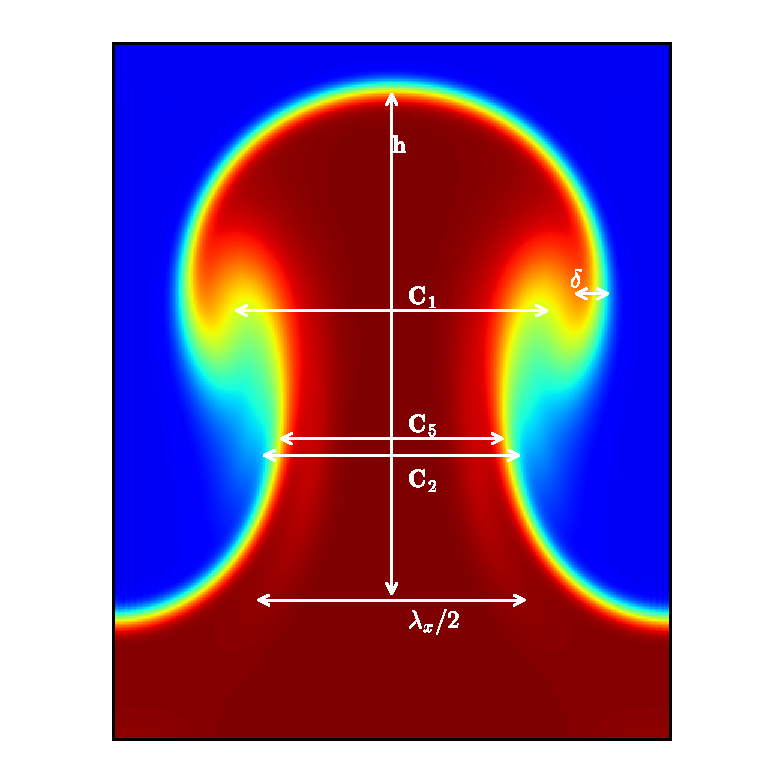
\includegraphics[width=\columnwidth]{figs/slice}
\caption{Scalar $\phi$}
\end{subfigure}
\begin{subfigure}[b]{\columnwidth}
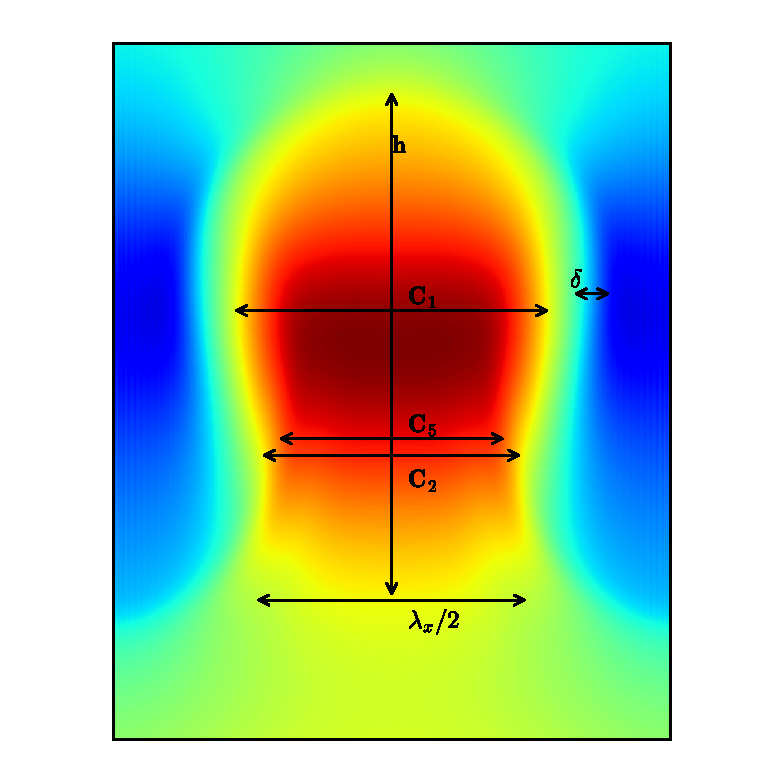
\includegraphics[width=\columnwidth]{figs/slice_w}
\caption{Vertical component of the velocity, $w$}
\end{subfigure}
\caption{
Slices of the scalar and vertical component of the velocity along the diagonal of a bubble at early times and high Rayleigh number.
The arrows indiciate the dependence of the model terms on different span-wise length scales, and are identical in both figures.
$C_1$ is related to the maximum cross sectional diameter of the bubble in the velocity field.
$C_2$ is related to the nominal side-wall diameter of the bubble in the velocity field.
$C_5$ is related to the nominal side-wall diameter of the bubble in the scalar field.
$\delta$ is related to the interface thickness in the scalar field.
}
\end{figure*}

The parameter $C_1$ scales the form drag and serves as a drag coefficient.  
Because we have let $C_0 = 1$, the hydralic diameter of the bubble is roughly $\lambda$.
Had we let $C_0 = 1/4$, the diameter would be the more common $\lambda/2$, but many of the parameters would be fractional.
Now, we relate $C_1$ to the drag coefficient $C_d$ in the drag equation:
\begin{equation}
C_1 \lambda^2 \dot{h}^2 = \frac{1}{2} C_d A \dot{h}^2
\end{equation}
so $C_1$ can be estimated using drag coefficients of similar objects:
\begin{equation} \elabel{prior_c1}
C_1 = \frac{C_d}{2} \frac{A}{\lambda^2}.
\end{equation}
Initially, the bubble tip is a flat plate, which has $C_d = 1.28$.
At late times, the bubble is closer to an elongated cylinder, which has $C_d = 0.82$, but with a somewhat streamlined tip, which further reduces drag.
We expect $C_1 \approx 0.64$, but possibly much smaller if the bubble takes a streamlined shape.
However, if the bubble spreads to have a diameter greater than $\lambda / 2$, $C_1$ could be greater than $0.64$.

Next, Consider the limit when $h \rightarrow \infty$ and $D = 0$:
The dynamical equation becomes
\begin{equation}
\ddot{h} = \frac{A g - C_2 \nu (1/\lambda) \dot{h}}{C_3}
\end{equation}
which leads to a terminal velocity of:
\begin{equation} \elabel{visc_vel}
\dot{h} = \frac{A g \lambda^2 }{C_2 \nu},
\end{equation}
or a non-dimensional velocity, i.e. Froude number:
\begin{equation}
\text{Fr} = \frac{d z}{d \tau} = \frac{\sqrt{\text{Gr}}}{C_2}.
\end{equation}
The case of extended bubbles and spikes affected only by viscous drag is highly analogous to flow through a square duct.
The pressure drop, $\Delta p$, along a duct is given by the Darcey-Weisbach formula:
\begin{equation}
\Delta p = \frac{f_D}{2} \frac{v^2 L}{d},
\end{equation}
where $L$ is the length of the duct,
$v$ is the mean velocity,
$d$ is the hydraulic diameter,
and $f_D$ is the Darcy friction factor.
In our case, $L = h$, $v = \dot{h}$, and $\Delta p = A g h$, so:
\begin{equation}
A g = \frac{f_D}{2} \frac{\dot{h}^2}{d},
\end{equation}
For laminar flows in circular pipes, $f_D = \bar{f}_D = 64 / \text{Re}$, so:
\begin{equation}
A g = \frac{f_D}{\bar{f}_D} 32 \nu \frac{\dot{h}}{d^2}.
\end{equation}
The hydraulic diameter $d = \lambda / 2$, so:
\begin{equation}
\dot{h} = \frac{\bar{f}_D}{f_D} \frac{A g \lambda^2}{128 \nu} .
\end{equation}
This gives an estimate for $C_2$:
\begin{equation}
C_2 \approx 128 \frac{f_D}{\bar{f}_D},
\end{equation}
where the ratio $f_D / \bar{f}_D$ is affected by the geometry and departure from laminar flow.
For example, for square ducts $f_D/\bar{f}_D \approx 0.889$, so $C_2 \approx 114.$. 

The product of the coefficient $C_5$ and $\lambda h$ gives the interfacial area of the side of the bubble.
If the bubbles were smooth and cylindrical, then $C_5 = \pi$
\begin{comment}
Next, consider the limit where $D = 0$ and $h \rightarrow 0$.
The dynamical equation becomes:
\begin{equation}
\ddot{h} = \left[\frac{C_0 A g }{C_3 \lambda} - C_2 \nu \dot{h}/\lambda \right] h
\end{equation}
In the spirit of the linear growth model, assume the interface grows as $h(t) = a_0 \cosh[\gamma t] $, with
\begin{equation}
\gamma = \frac{C_0 A g }{C_3 \lambda} - C_2 \nu \dot{h}/\lambda 
\end{equation}
The velocity is given by $\dot{h} = a_0 \gamma \sinh[\gamma t] = \gamma \tanh[\gamma t] h$, yielding:
\begin{equation}
\gamma = \frac{C_0 A g }{C_3 \lambda} - \gamma C_2 \tanh[\gamma t] h \nu /\lambda 
\end{equation}
\end{comment}
